Consider the KNighter-derived CSA checker for Linux commit
\texttt{5aa2184e2908}, which fixes a double-free error path in
\lstinline|mlx5hws_definer_calc_layout|~\cite{linuxCommit5aa2184e,yang2025knighter}.
Figure~\ref{fig:motivating} shows two fallible calls: conversion helper
\lstinline|hws_definer_conv_match_params_to_hl| (\cmark{1}) establishes
ownership of \lstinline|mt->fc| only on success; a later layout-fitting
failure may then legitimately release it through \lstinline|free_fc|.
On conversion failure, however, the vulnerable \lstinline|goto| targets
\lstinline|free_fc| (\cmark{2}) before ownership exists.  The patch
redirects only that edge to \lstinline|free_match_hl| (\cmark{4}),
which frees the already-owned \lstinline|match_hl| while bypassing
\lstinline|mt->fc|.  The needed predicate distinguishes these guarded
error paths, not merely the presence of a free call.

% Current figure design:
%   Panel A: patch hunk with M1--M21 labels.  Solid arrows are real patch
%   control flow; dashed arrows are checker-to-code mappings.  Orange marks the
%   unsafe/report path, teal marks the refined/barrier path, and gray marks
%   generic scanning or legitimate later control flow.
%   Panel B: baseline broad allocation/free checker with B1--B14 labels and
%   strict-validation outcome 10/9.
%   Panel C: refined path/state predicate with C1--C15 labels and
%   strict-validation outcome 1/0.
\begin{figure*}[t]
  \centering
  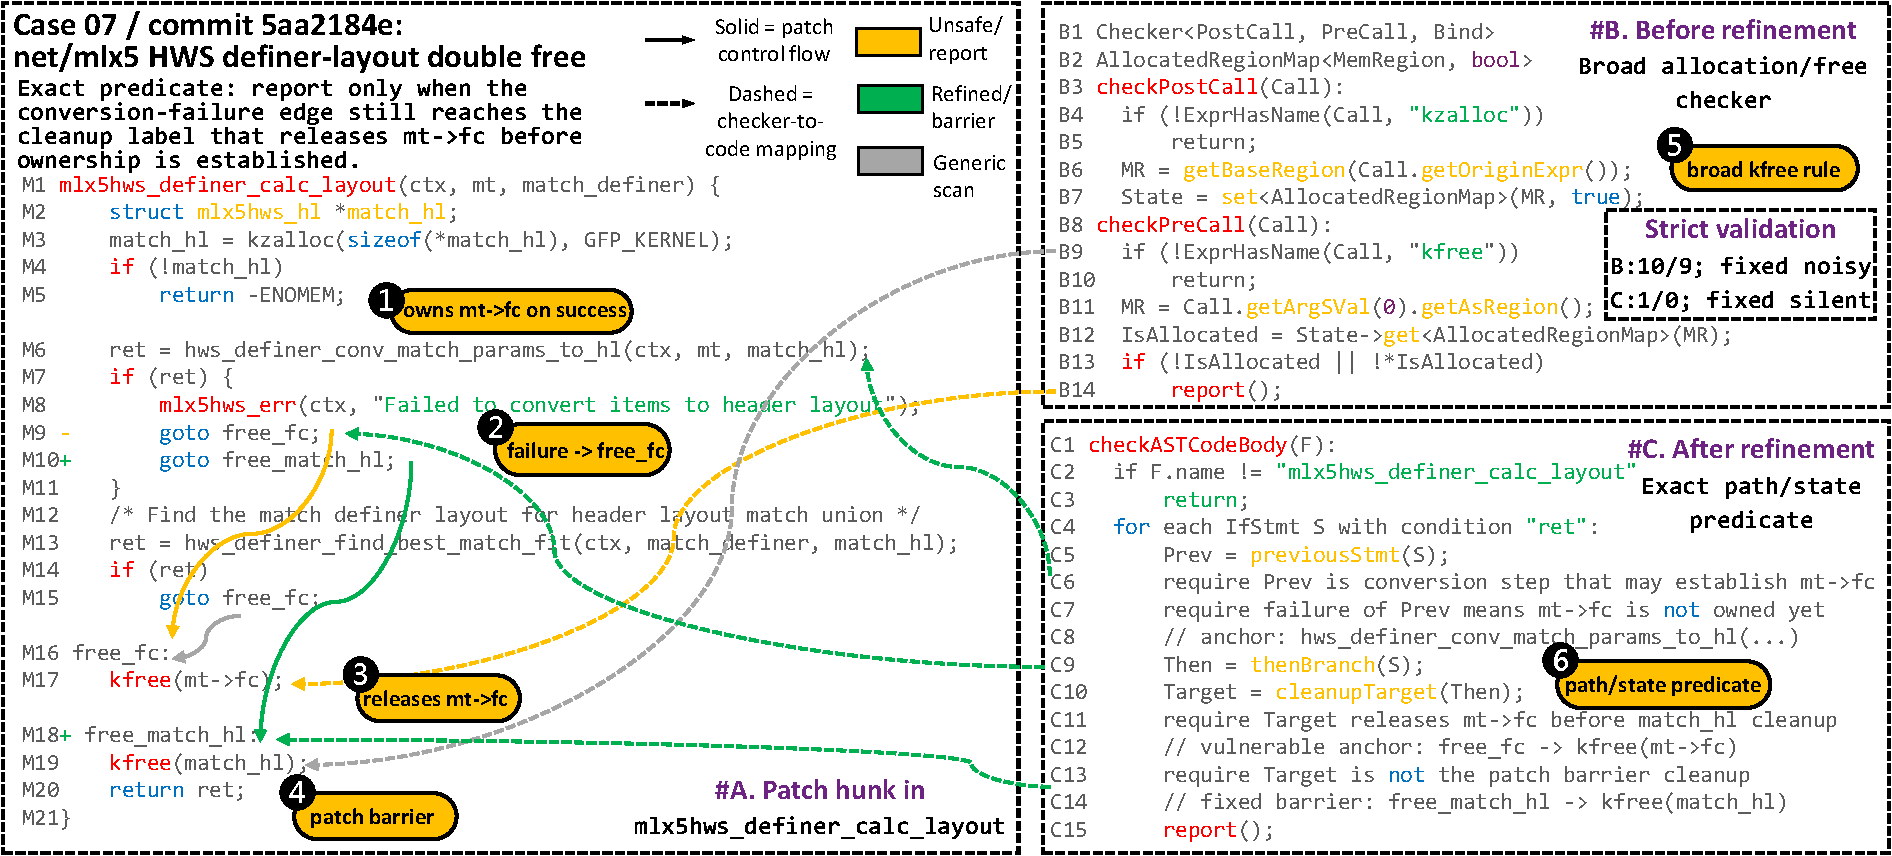
\includegraphics[width=\textwidth]{figures/fig-motivating.pdf}
  \Description{Three-panel example showing the vulnerable and fixed cleanup edges, the broad starting checker with ten and nine alerts, and a manually completed patch-bound checker with one and zero alerts.}
  \caption{\textbf{Motivating double-free refinement.}
  Solid arrows show patch control flow. Dashed arrows show
  checker-to-code mappings.  Orange highlights the unsafe path,
  teal the patched barrier, and gray the legitimate later flow.
  The baseline checker (\cmark{5}) fires broadly (\texttt{10/9}).
  The manually completed checker (\cmark{6}) encodes the conversion-failure
  ownership predicate and achieves \texttt{1/0}; this case is not an
  automatic-refinement success.}
  \label{fig:motivating}
\end{figure*}

\textbf{Checker behavior and evidence.}
The starting checker (\cmark{5}) tracks \lstinline|kzalloc| regions
and warns at \lstinline|kfree| when a region is absent from its map.
It misses the guarded ownership distinction and emits \texttt{10/9}
patch-local alerts on vulnerable/fixed revisions.  A fixed-side report
shows the symptom but does not identify the conversion call, guard,
cleanup edge, and owned object that form the separator.  The evidence
bundle places the two cleanup labels and guarded edges in one semantic
slice; a Clang CFG dump supports branch context, while the ownership
interpretation comes from patch and source analysis, \emph{not} a
path-feasible analyzer proof.  A validation-only edit can simply suppress
both sides: the historical one-run ablation here produced \texttt{0/0}.

The checker in Figure~\ref{fig:motivating}c was \emph{manually completed}:
its AST-body predicate recognizes the conversion-failure edge and changes
paired counts to \texttt{1/0}.  It is not an automatic \toolname success.
Modeling the allocator or tracked-state check in the original symbolic
checker would be another plausible repair; this example does not show
that the AST rewrite is preferable.  The shown predicate names the patch
function and is therefore patch-bound, not a general double-free detector.
The strict PDS gate establishes only the paired result, not stability
under future changes to the code or callback names.
